\section{Introduction}
\label{sec:introduction}

% % Underwater Robot Applications:
%
%Operating in complex, hazardous, and otherwise inaccessible environments, \Acfp{ROV} have become essential for a diverse range of demanding applications, including surveying, infrastructure inspection, and search-and-rescue, significantly expanding operational possibilities~\cite{amer2023unav, amer2025modelling}.
%
% Why We Need Tether:
%
%Most \acp{ROV} are tethered to ensure a continuous power supply during long-duration missions and to maintain reliable communication.

Remotely operated vehicles \Acfp{ROV} have become essential for operations in complex, hazardous, and otherwise inaccessible environments. They facilitate a diverse range of demanding applications, including surveying, infrastructure inspection, and search and rescue missions, thus significantly expanding operational possibilities \cite{amer2023unav, amer2025modelling}. Most \acp{ROV} are tethered to a host platform to maintain reliable communication and ensure a continuous power supply during long-duration missions. However, this tethering infrastructure introduces operational challenges related to planning and control while posing the risk of being entangled with underwater objects such as flora, fauna, or structures under inspection.

%
% Introducing Problem Definition:
%
%However, the presence of a tether introduces complexities in path planning and control, as it poses a risk of entanglement with underwater objects such as flora, fauna, or the underwater structures being inspected.

%Tether-related challenges restrict the applicability of path-planning algorithms originally designed for untethered systems. For instance, numerous \ac{CPP} algorithms exist to compute distance-optimal paths for covering 3D structures \cite{bircher2015structural,feng2024fc, amer2023visual}. Additionally, exploration path planners are employed to determine the next viewpoints for mapping and exploring unknown terrains \cite{dang2020graph}. However, these methods do not account for entanglement with the surroundings and thus cannot be directly applied to tethered underwater robots.

Numerous \ac{CPP} algorithms are proposed in the literature for inspection-related tasks with untethered systems. In essence, they compute distance-optimal paths for a thorough inspection of 3D structures \cite{bircher2015structural,feng2024fc, amer2023visual}.  Additionally, exploration path planners are employed to determine the next viewpoints for mapping unknown terrains \cite{dang2020graph}. However, these path-planning methods are restricted to untethered systems, as they do not account for possible entanglements with the surroundings. Hence, the literature still lacks path-planning algorithms that directly address tether-related challenges.

%
% Entanglement Problem and Definition:
%
In case of underwater inspection, entanglement occurs when the vehicle's movement is restricted due to interaction between the tether and objects in the environment. The tether can loop around obstacles, thereby limiting the vehicle's mobility and substantially reducing operational range in a worst-case scenario. Consequently, operators need to carry longer tethers to account for possible entanglements without a proper planner at hand.
In this work, we propose the \ac{REACT} algorithm that fills this critical gap in underwater asset inspection. In essence, when integrated into the coverage path planning framework, \ac{REACT} renders entanglement-free paths, thus ensuring task completion without the need to carry additional tether lengths. Besides, the proposed planning framework reduces overall operational time by circumventing the post-completion detangling process, often required with traditional path-planning methods. The contributions of this work can be summarized as follows:
\begin{itemize}
\item A fast tether model that computes the tether configuration in real-time using \ac{SDF} data of arbitrary underwater structures.
\item An efficient online replanning method \ac{REACT} that prevents entanglement by incorporating a tether-length constraint.
%\item Integration of the proposed method into a \ac{CPP} framework with \ac{MPC} to enable optimal inspection while avoiding entanglement.
\item \ac{REACT}'s integration with an off-the-shelf \ac{CPP} along with \ac{MPC}, rendering optimal trajectory following.
\item Demonstration of the framework in simulation and real-world tests, showcasing its ability to ensure safe and time-efficient inspection.
\end{itemize}


%
\begin{figure}[t!]
	\centering	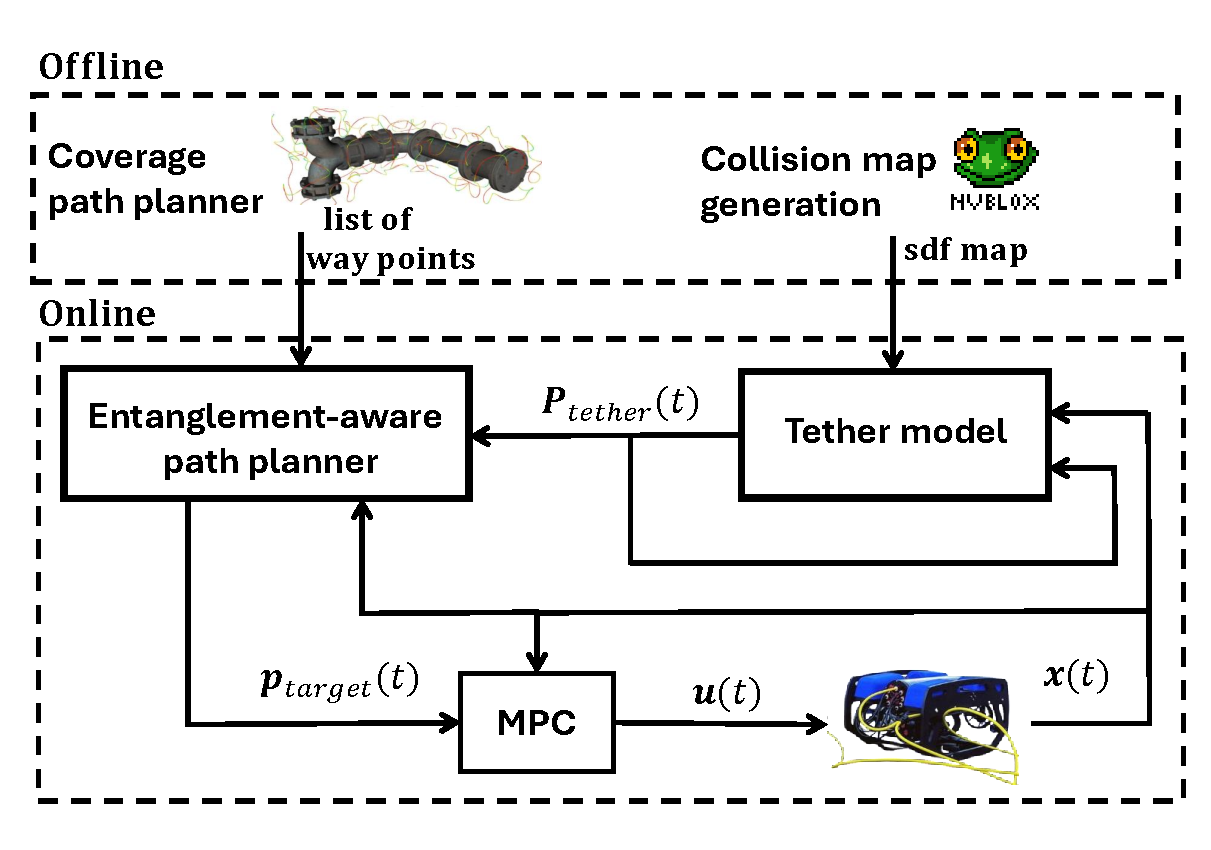
\includegraphics[width=1\linewidth]{EA-Planner/figures/abstract.pdf}
	  \caption{\textcolor{black}{Overview of the \ac{REACT} inspection framework. Offline, a \ac{SDF} map is generated from a point cloud, and an off-the-shelf \ac{CPP} \cite{feng2024fc} is used to compute an optimal waypoint sequence. During operation, a tether model $(\mathbf{P}_{tether}(t))$ is used  to ensure tether length is not exceeded, while an \ac{MPC} controller applies the optimal wrench $\mathbf{u}(t)$ to the \ac{ROV}}.}
    \label{fig:abstract}
\end{figure}
%







The remainder of this paper is organized as follows: Section \ref{sec:related_work} reviews the state of the art. Section \ref{sec:framework} presents the path planning framework for underwater structure inspection with tether constraints. Section \ref{sec:tether_model} introduces the taut-tether model, and Section \ref{sec:planner} details the online entanglement-aware path planner. Experimental results are presented in Sections \ref{sec:simulationexperiments} and \ref{sec:real-world}, followed by conclusions in Section \ref{sec:conclusion}.





